\documentclass[../main.tex]{subfiles}
\makeatletter
\@ifundefined{fromRoot}{%
  \newcommand{\fromRoot}[1]{../#1}
  
  \usepackage{xr}
  \externaldocument{../main}
}{}

\def\input@path{{\subfix{../}}}
%or: \def\input@path{{/path/to/folder/}{/path/to/other/folder/}}
\makeatother

\graphicspath{{\subfix{../}}}

\hypersetup{
    pdfauthor   = {Mael Tourres},
    pdftitle    = {Th\`{e}se (Chapitre 3_2)},
    pdfsubject  = {Th\`{e}se (Chapitre 3_2)},
%    pdfkeywords = {mots-cl\'{e}s},
}

\begin{document}
\selectlanguage{french}
%
%
%
%
%
\chapter{Extensions SIMD pour l'accélération des décodeurs de CCE} 
\label{chapter:3_2}
\chaptermark{Extensions SIMD pour l'accélération des décodeurs de CCE}

Dans ce chapitre, l'amélioration des instructions scalaires opérant sur des données codées sur 8 bits vers des instructions de type SIMD afin d'exploiter l'architecture 32 bits des processeurs est détaillée. 
L'objectif est alors de permettre une montée en débit des décodeurs logiciels grâce aux stratégies de parallélisation utilisées dans la littérature.
De manière analogue à l'intégration des instructions scalaires, les résultats issus du prototypage sur cible FPGA des processeurs RISC-V enrichis évaluent l'impact des propositions sur le débit et la complexité.

Il est à noter que dans ce chapitre, comme pour le précédent, nous étudierons des architectures à 2 registres d'entrée et un registre de sortie. Ce format correspond au format standard des jeux d'instructions des processeurs x86 (Intel, AMD), \acrshort{risc} et dérivés (ARM) et RISC-V. Une étude exploitant des architectures levant en partie cette restriction sera présentée dans le chapitre suivant.

\etocsetnexttocdepth{4}
\etocsettocstyle{{\large \hspace{-1.5 em} \textbf{} \hfill}\vspace{-2.5 em}\\\par\noindent\rule{\linewidth}{1 pt}\vspace{-.2 em}}{\par\noindent\rule{\linewidth}{1 pt}\\}
\localtableofcontents
%
%
%
%\section{Extension des instructions en mode SIMD}
%
%
% 
% 
\section{Introduction}
% 
%
% 
% 
L'étude et les expériences précédentes se sont focalisées sur des instructions de type SISD. Toutefois, dans la littérature, les décodeurs logiciels tirent parti des fonctionnalités SIMD des architectures multicœurs actuelles pour atteindre des niveaux de performances élevés. Ainsi, l'extension des instructions scalaires sur 8 bits vers des vecteurs de $Q \times 8$ bits est étudié et évalué dans cette section. Comme cela a été introduit dans le chapitre précédent, les décodeurs de CCE manipulent des données sur 8 bits. L'architecture interne des processeurs modernes, de leur chemin de données à leurs registres, sont sur 32 bits, voir 64 bits. Ainsi il est théoriquement possible sur des architectures 32 bits de traiter jusqu'à quatre données en parallèle en un même cycle d'horloge si les formulations des algorithmes le permettent.
%%%%%%%%%%%%%%%%%%%%%%%%%%%%%%%%%%%%%%%%%%%%%%%%%%%%%%
\begin{figure}[!tb]
	\centering
	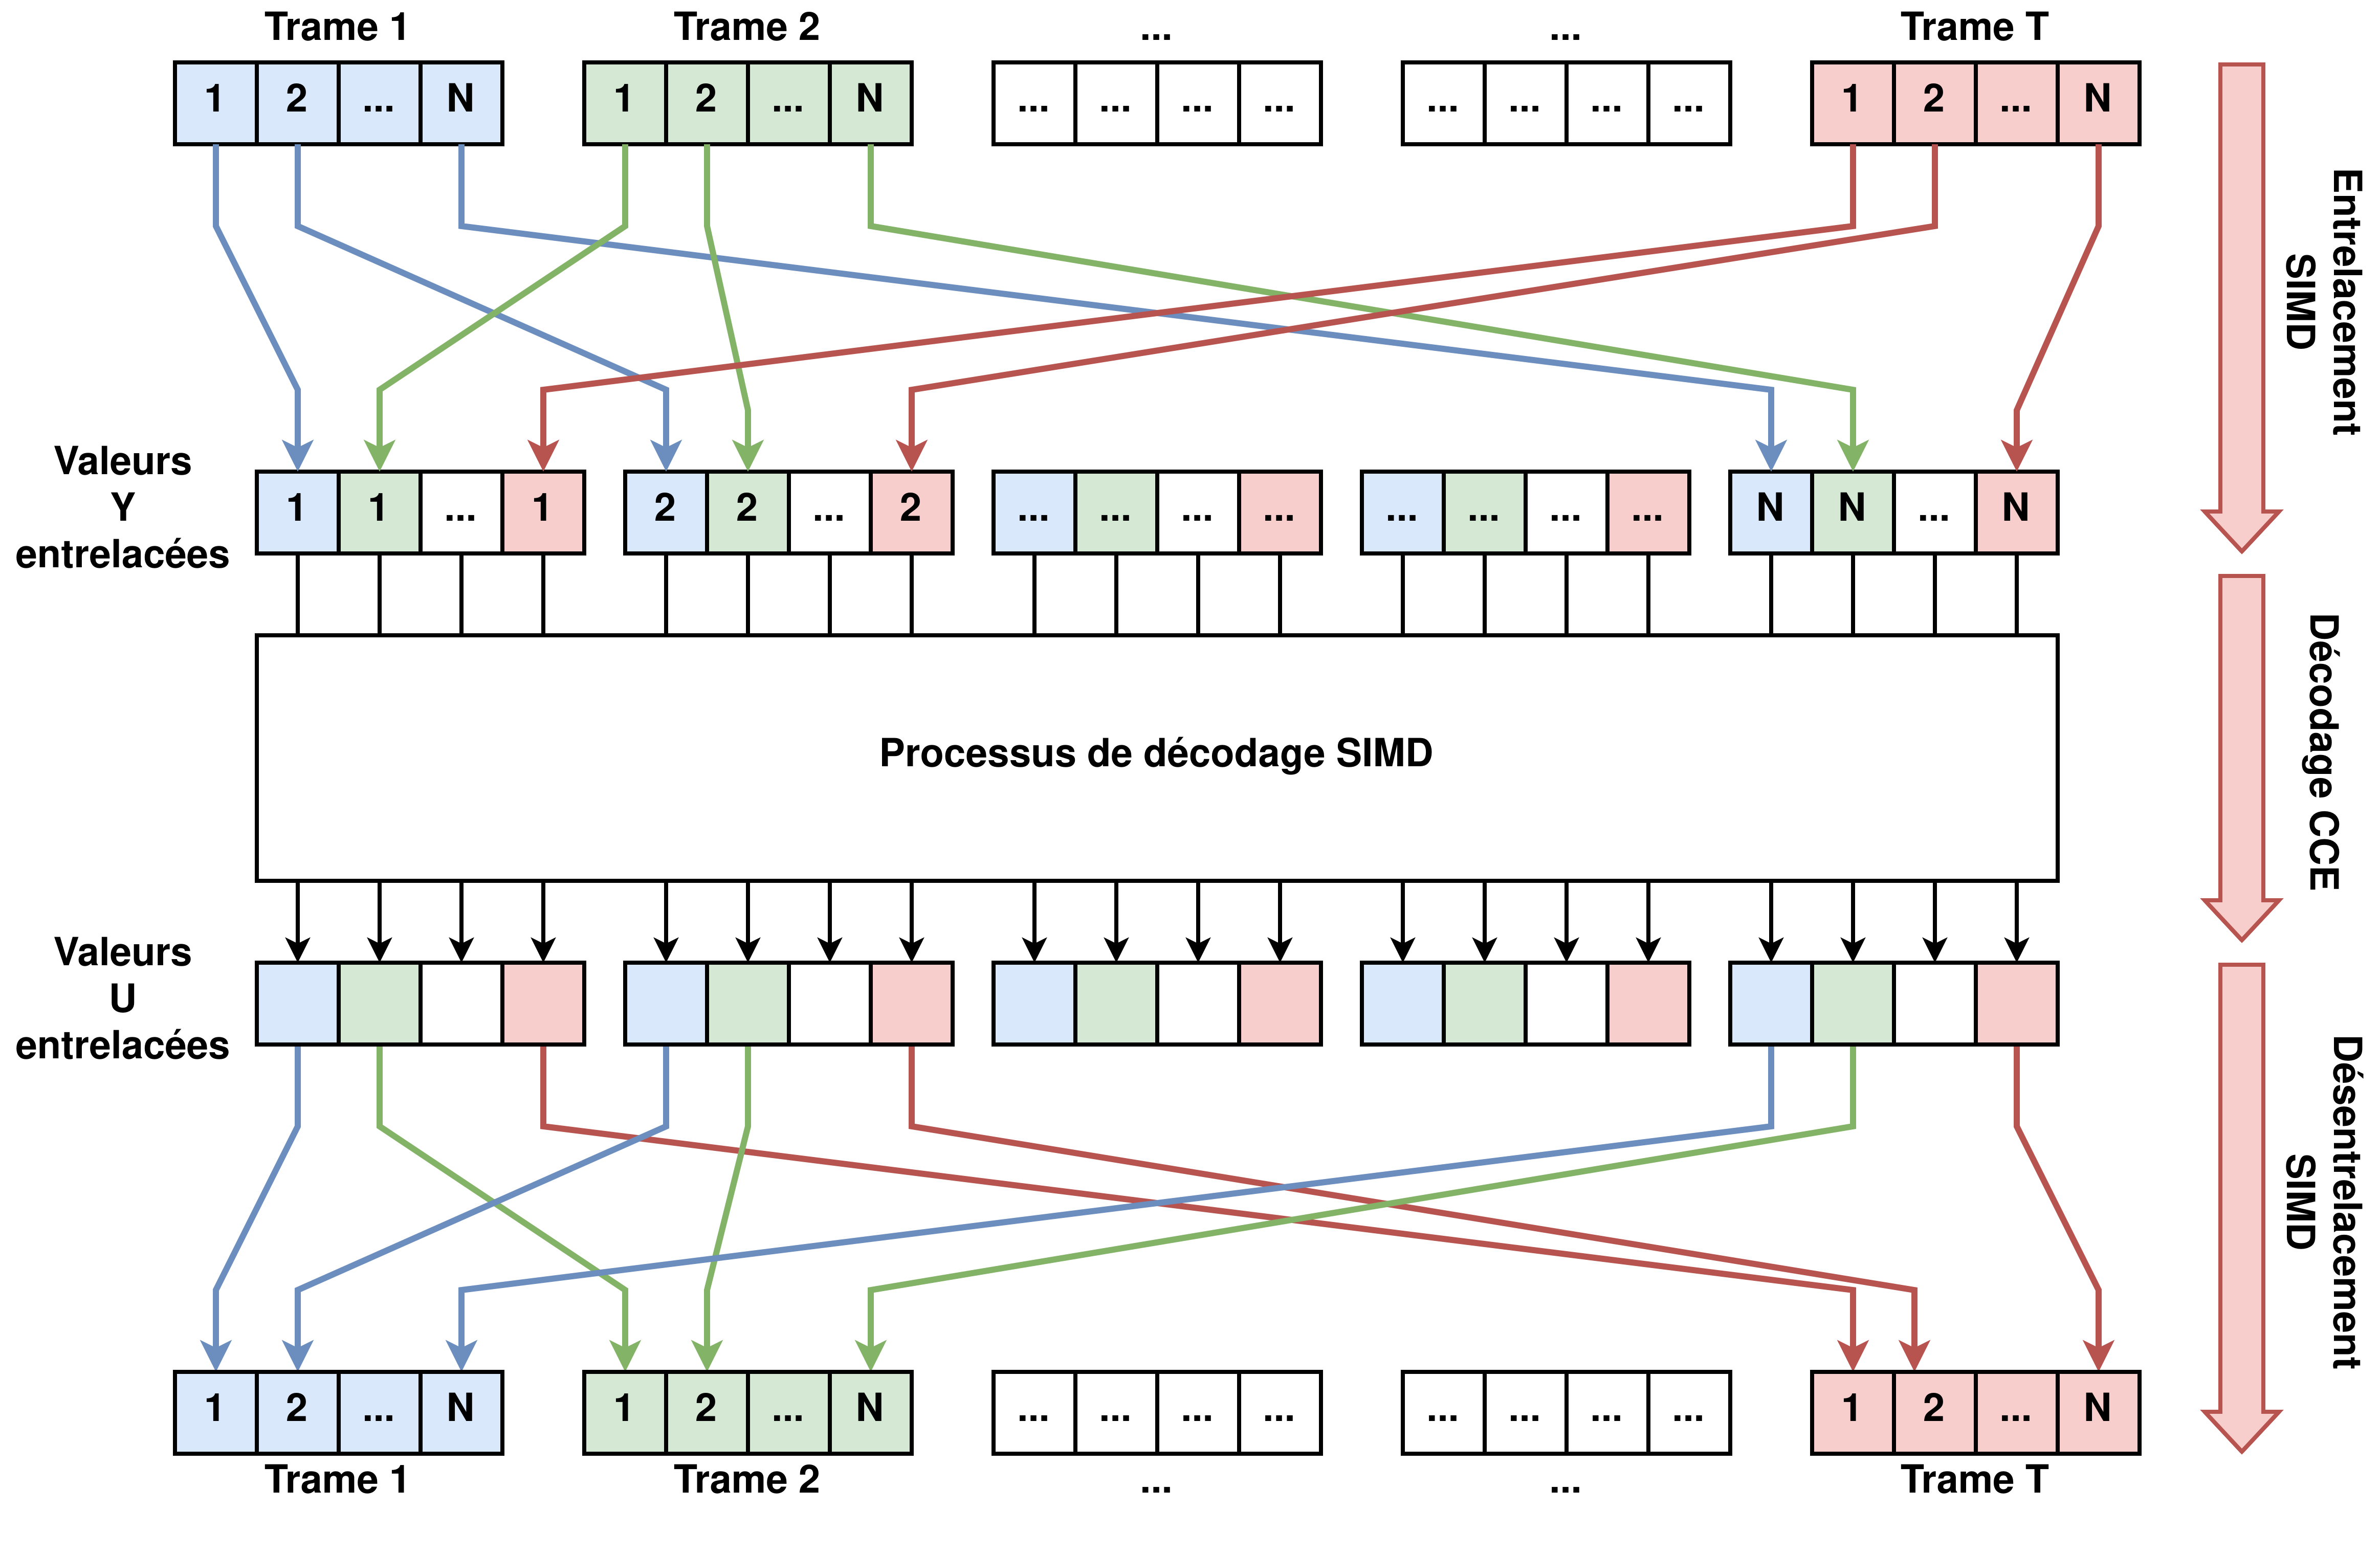
\includegraphics[scale=.08]{figs/SIMD.png}
	\caption{Approche de la parallélisation inter-trames incluant les étages d'entrelacement dans l'ordre et inverse.}
	\label{process_SIMD}
\end{figure}
%%%%%%%%%%%%%%%%%%%%%%%%%%%%%%%%%%%%%%%%%%%%%%%%%%%%%%
Le schéma de parallélisation inter-trames consiste à répliquer les mêmes opérations de décodage sur plusieurs trames indépendantes afin de mettre en exergue un parallélisme de calcul facilement accessible. 
Cela permet d'augmenter le débit des architectures au prix de faibles modifications dans les codes algorithmiques. 
Cette parallélisation inter-trames a été utilisée à l'origine dans des travaux relatifs à l'accélération des décodeurs CCE sur des architectures multicœurs \cite{Adrien,ri:LeG19c,LDPC:SOFT4}. 
Toutefois, afin de faciliter les accès mémoires et maximiser l'utilisation des unités de calcul SIMD, les données doivent être arrangées correctement dans la mémoire. 
Un entrelacement des données contenues dans les différentes trames est réalisé en amont du processus de décodage, tel que cela est schématisé dans la figure \ref{process_SIMD}. 
Pour maintenir le comportement du système, à la fin de chaque décodage, l'opération inverse est exécutée. 
Comme cela a été rapporté dans \cite{LDPC:SOFT4}, le temps d'exécution des ces étapes d'entrelacement des données est négligeable par rapport au temps d'exécution des processus de décodage ces CCE.

À l'opposée de cette stratégie de parallélisation inter-trames opérant sur des jeux de données différents, la parallélisation intra-trame vise à exploiter le parallélisme de calcul interne à l'algorithme de décodage, tel que cela est mis en œuvre dans l'intégralité des décodeurs de CCE matériels. 
Cette approche permet de réduire fortement la complexité mémoire, car le processus de décodage ne mémorise et ne traite qu'une trame à la fois. 
Cela permet aussi de réduire la latence de traitement. 
Cependant, d'un point de vue logiciel, la formalisation de tels décodeurs est plus complexes à réaliser que pour l'approche inter-trames.

Dans tous les cas, comme cela a été démontré dans la littérature, les formulations algorithmiques permettant de tirer parti des spécificités architecturales tel que les unités SIMD sont plus complexes à décrire. 
De plus, les facteurs d'accélération n'évoluent pas toujours linéairement avec la taille des unités SIMD.


%%%%%%%%%%%%%%%%%%%%%%%%%%%%%%%%%%%%%%%%%%%%%%%%%%%%%%
\begin{table}[!tb]
    \scriptsize
    \centering
  
    \begin{tabular}{llccc}
        \toprule
        \multirow{2}{*}{\textbf{CCE}} & \multirow[c]{2}{*}{\textbf{Mnemonic}} &  \textbf{SISD} 
        &\textbf{SIMD Inter}
        &\textbf{SIMD Intra}\\
        & & (int8) & (int8x4) & (int8x4) \\ 
        \toprule
  
  \multirow{1}{*}{LDPC}
          % LDPC 
          &   i8\_abs\_pi8           &  \checkmark  &   \checkmark  &   \checkmark  \\
          &   i8\_add\_sat127\_pi8   &  \checkmark  &   \checkmark  &   \checkmark  \\
          &   i8\_invB\_Aneq1\_pi8   &  \checkmark  &   \checkmark  &               \\
          &   i8\_xorA\_signB\_pi8   &  \checkmark  &   \checkmark  &               \\
          &   i8\_cmpeq\_pi8         &  \checkmark  &   \checkmark  &  \checkmark   \\
          &   i8\_max\_pi8           &  \checkmark  &   \checkmark  &  \checkmark   \\
          &   i8\_min\_pi8           &  \checkmark  &   \checkmark  &               \\
          &   i8\_sub\_sat127\_pi8   &  \checkmark  &   \checkmark  & \checkmark    \\
          &   i8\_sign\_pi8          &              &   \checkmark  &               \\
          &   i8\_cpysign\_pi8       &              &               &  \checkmark   \\       
          &   i8\_signextract\_pi8   &              &               &  \checkmark   \\               
          \cmidrule(l){1-5}
  
  \multirow{1}{*}{polaire}    
          &  i8\_add\_sat127\_pi8   &  \checkmark   & \checkmark    & \checkmark   \\        
          &  i8\_sub\_sat127\_pi8   &  \checkmark   & \checkmark    & \checkmark   \\
          &  i8\_Fx\_pi8            &  \checkmark   & \checkmark    & \checkmark   \\
          &  i8\_Rx\_pi8            &  \checkmark   & \checkmark    & \checkmark   \\
          &  i8\_clrA\_Bneq0\_pi8   &               & \checkmark    & \checkmark   \\
          &  i8\_setMask\_Aeq1      &               & \checkmark    & \checkmark   \\
          \cmidrule(l){2-5}
            
  \multirow{1}{*}{+ F-SC}
          &  i16\_add\_accA\_loB\_pi8   &           & \checkmark    &   \\        
          &  i16\_add\_accA\_hiB\_pi8   &           & \checkmark    &   \\        
          &  i8\_sign\_pi16             &           & \checkmark    &       \\    
          &  i8\_Hxor\_pi8              &           &               &  \checkmark   \\        
          &  i8\_Hadd\_pi8              &           &               &  \checkmark  \\   
          \cmidrule(l){1-5}     
    
  \multirow{1}{*}{LDPC-NB}
          % ldnb 
          & u8\_minu\_pu8               &   \checkmark   & \checkmark &  \checkmark    \\        
          & u8\_addu\_sat64\_pu8        &   \checkmark   & \checkmark &  \checkmark    \\
          & u8\_subu\_sat64\_pu8        &   \checkmark   & \checkmark &  \checkmark    \\
          % inter 
          & u8\_cmpge\_pu8              &       & \checkmark &       \\
          & u8\_Aandb\_lo8B\_pu8        &       & \checkmark &       \\
          & u8\_maxu\_pu8               &       & \checkmark &       \\
          % intra 
          & u8\_hminu\_pu8              &       &   & \checkmark     \\
          \cmidrule(l){1-5} 
          
\multirow{1}{*}{turbo}
          &  i8\_max\_pi8               &   \checkmark      & \checkmark        &  \checkmark   \\       
          &  i8\_scale\_pi8             &   \checkmark      & \checkmark        &               \\
          & i8\_add\_pi8                &                   &  \checkmark       &  \checkmark   \\
          & i8\_sub\_pi8                &                   &  \checkmark       &  \checkmark   \\
          & i8\_add\_srl\_pi8           &                   &  \checkmark       &               \\ 
          & i8\_srl1\_pi8               &                   &  \checkmark       &               \\
          & i8\_sign\_pi8               &                   &  \checkmark       &               \\
          & i8\_shuffle\_pi8            &                   &                   &   \checkmark  \\
          & i8\_srl\_pi8                &                   &                   &   \checkmark  \\
          & i8\_min\_pi8                &                   &                   &   \checkmark  \\
  
          \bottomrule
      \end{tabular}   
      \caption{Liste des instructions spécifiques avec Mnemonic et compabilité SISD/SIMD.}
      \label{liste:all:instr}
  \end{table}
%%%%%%%%%%%%%%%%%%%%%%%%%%%%%%%%%%%%%%%%%%%%%%%%%%%%%%
\begin{table}
    \centering
    \footnotesize
    \begin{tabular}{lccc}
        \toprule
        \multirow{2}{*}{\textbf{CCE}}&  \textbf{SISD} & \textbf{SIMD Inter} & \textbf{SIMD Intra}     \\
                            & (int8)&(int8x4)   & (int8x4)      \\
        \toprule
        LDPC                & 8     & 9         & 7             \\
        \cmidrule(l){2-4}
        polaire             & 4     & 6         & 6             \\
        \cmidrule(l){2-4}
        polaire F-SC        & 4     & 9         & 8             \\
        \cmidrule(l){2-4}
        LDPC-NB             & 3     & 6         & 4             \\
        \cmidrule(l){2-4}
        turbo               & 2     &  7        & 6             \\
        \bottomrule
    \end{tabular}
    \caption{Synthèse du nombre d'instructions identifiées par famille de CCE.}
    \label{sum:all:instr}
\end{table}
%%%%%%%%%%%%%%%%%%%%%%%%%%%%%%%%%%%%%%%%%%%%%%%%%%%%%%

Pour pouvoir utiliser l'ensemble de ces stratégies de parallélisation, il est nécessaire d'étendre le jeu d'instructions pour pouvoir gérer par exemple les opérations conditionnelles. 
En effet, lors des traitements SIMD, les mêmes traitements sont appliqués à l'ensemble des données, rendant de fait impossible l'utilisation de structure de type $if$ permettant d'inverser par exemple le signe d'une donnée en fonction d'un calcul de parité. 
Pour palier à cela, des instructions spécifiques ont été ajoutées à la liste des opérations scalaires dédiées déjà identifiées. 
La liste exhaustive des extensions nécessaires aux descriptions SIMD est fournie dans le tableau \ref{liste:all:instr}.
Ce tableau indique pour chaque instruction son usage en fonction des stratégies de parallélisation. 
La description des traitements réalisés par ces instructions a été placée en annexe pour des raisons de lisibilité. 
L'ensemble des descriptions logicielles des décodeurs CCE ont été retravaillées afin d'exploiter ces instructions et offrir des stratégies de parallélisation inter et intra-trame. 
Un résumé du nombre d'instructions par famille de code et schéma de parallélisation est fourni dans le tableau \ref{sum:all:instr}. 
Dans la suite de ce chapitre, les résultats obtenus sont présentés.

% 
% 
% 
% 
% 
\section{Expérimentations menées sur des décodeurs SIMD inter-trames}
% 
% 
% 
% 
% 

L'évaluation conduite s'est d'abord portée sur le schéma de parallélisation inter-trames. 
Ce choix est lié au fait que les modifications à apporter aux descriptions logicielles sont moins conséquentes que de basculer vers un schéma de parallélisation intra-trame.
Les cœurs de processeur RISC-V étudiés étant des cœurs 32 bits, il était ainsi naturel de sélectionner un format SIMD de type \textit{int8\_t \times 4} sachant que les décodeurs manipulent naturellement des données sur 8 bits. 
Ce format SIMD permet le traitement de 4 données en parallèle par cycle d'horloge, et par voie de conséquence autorise 4 trames à être décodées de manière simultanée. 
Les opérations appliquées sur les 4 trames étant identiques, il est alors possible d'assurer une utilisation maximale des ressources de calcul.

Les résultats expérimentaux concernant le temps d'exécution des différents décodeurs sont reportés dans la table \ref{cycles_bit_simd_inter} et \ref{tab:cycles_inter_2r_p1} et \ref{tab:cycles_inter_2r_p2}.
Ces résultats sont comparés à ceux obtenus précédemment lorsque les instructions spécialisées manipulaient des instructions scalaires (SISD) (\textit{\ding{183} SISD}) et également avec les décodeurs de base sans l'aide d'instructions spécialisées \textit{\ding{182} Baseline}.
Les données présentées montrent qu'en moyenne, les instructions SIMD ajoutées permettent de réduire de $75\%$ le temps de décodage des bits par rapport à la solution incorporant nos instructions SISD. 
Les débits sont également considérablement améliorés lorsqu'ils sont comparés avec la baseline et les instructions SISD.
Ce constat est cohérent avec la stratégie de parallélisation employée, même s'il est difficile d'expliquer précisément les raisons des légères disparités entre les versions d'un même décodeur sur les différentes architectures.

Si l'on analyse dans un premier temps les codes CCE et que l'on regarde les décodeurs LDPC binaires et non binaires, le problème ne se pose pas.
En effet, les gains avoisinent $75\%$ et les débits sont améliorés d'un facteur supérieur à $6\times$ sur toutes les architectures. 
Cela s'explique par le fait que ces algorithmes sont composés de nids de boucles et sont donc réguliers dans leur flot d'exécution.

Les codes polaires utilisent la récursivité durant le décodage, engendrant des appels de fonction non accélérés par les instructions SIMD introduites. 
En conséquence, les gains observés sont moindres, variant de $\approx 66\%$ (\IBEX , \RISCY ) à $70\%$ (\SCR) en réduction de cycles/bit et de $4.4\times$ à $5.3\times$ en débit. 
Les codes polaires avec l'algorithme Fast-SC présentent des gains moindres, variant de $63\%$ à $\approx 59\%$ en cycles/bit également, et les débits varient de $4.1\times$ à $4.9\times$. 
En effet, dans cet algorithme, la simplification de séquences d'instructions est plus ardue du fait de nœuds très spécifiques (\textit{REP, SPC}). 
Ces nœuds comportent des opérations qui ne sont pas réductibles à des instructions spécialisées.
Par exemple, les nœuds \textit{SPC} nécessitent une recherche de minima avec leur position associée dans leurs versions inter-trames. 
Ces opérations conditionnelles sont plus simples à approcher avec une donnée unique, mais deviennent plus complexes à implanter avec 4 données distinctes.  

Les turbo codes présentent une réduction des cycles nécessaires au décodage d'un bit de donnée en moyenne de $70\%$, conformément aux résultats attendus avec des débits variant de $3.8\times$ à $4.5\times$. 

En conclusion, d'un point de vue applicatif on peut noter qu'indépendamment de la famille de code testée, les versions inter-trames SIMD déployées sur les cœurs offrent systématiquement une réduction significative de $\approx 70\%$ en nombre de cycles nécessaires au décodage d'un bit et des débits augmentant d'un facteur de $5\times$ en moyenne.
%%%%%%%%%%%%%%%%%%%%%%%%%%%%%%%%%%%%%%%%%%%%%%%%%%%%%%
\begin{table}[!tb]
    \footnotesize
    \centering
    \begin{tabular}{@{}lllrrrrr@{}}
        \toprule
        & & & \textbf{LDPC}  & \multicolumn{2}{r}{\textbf{polaire}}           & \textbf{LDPC-NB}       & \textbf{turbo} \\
        & & & OMS   & SC                    & F-SC          & MS            & MLM  \\ 
        \midrule  

        \multirow{2}{*}{\PicoRV}& 
        \multirow{2}{*}{Cycles/Bit} 
        &    SISD   & 484       & 91        & 40            & 11 234         & 202     \\
        &  & SIMD   & -76.9\%   & -68.2\%   & -62.3\%       & -72.5\%       &  -70.8\% \\
        \cmidrule(l){2-8}

        \multirow{2}{*}{\IBEX}&
        \multirow{2}{*}{Cycles/Bit} 
        &   SISD    & 199       &     35    &16             & 4 245          & 63 \\
        & & SIMD    &  -76.1\%  &  -65.9\%  &-58.9\%        &  -72.2\%      & -70\%\\ 
        \cmidrule(l){2-8}

        \multirow{2}{*}{\SCR}& 
        \multirow{2}{*}{Cycles/Bit} 
        &       SISD  & 172     & 34        & 15            & 4 226         &  61.3\\
        &  &    SIMD  &-76.7\%  &-70.6\%    &-63.1\%        &  -72.6\%      &  -70.5\%\\
        \cmidrule(l){2-8}

        \multirow{2}{*}{\RISCY}&
        \multirow{2}{*}{Cycles/Bit} 
        &   SISD    & 176       & 28        & 13            & 948           & 54 \\
        & &  SIMD   & -76.4\%   & -65.6\%   & -58.8\%       & -72.4\%       & -70\% \\
        \bottomrule 
    
    \end{tabular}
    \caption{Réduction du nombre de cycles d'horloge nécessaire au décodage d'un bit grâce à l'usage des instructions SIMD dédiées - Stratégie de parallélisation inter-trames.} 
    \label{cycles_bit_simd_inter}
\end{table}
%%%%%%%%%%%%%%%%%%%%%%%%%%%%%%%%%%%%%%%%%%%%%%%%%%%%%%
\begin{table}[!tb]
    \footnotesize
    \centering
    \begin{tabular}{lllrrrrr} %8
    \toprule
    &  &    & \textbf{LDPC}  &       & \textbf{polaire}   & \textbf{LDPCNB}   & \textbf{turbo} \\ 
    &  &    & OMS   & SC    & F-SC      & MS        & MLM   \\
    \cmidrule(l){1-8}
    \PicoRV
    & \ding{182} Baseline                       & cycles    & 217172 & 1333324 & 676218 & 3476435 & 2503511    \\
    \cmidrule(l){2-8}
    
    & \ding{183} SISD                    & cycles    & 131853 & 753144 & 332693 & 2875953 & 2133442     \\
    & \ding{184} SIMD INTER             & cycles    & 122462 & 916029 & 502106 & 3166507 & 2488956     \\
    \cmidrule(l){2-8}
    
    & Gain (\ding{182}\rightarrow\ding{183})    & cycles    & 85319 & 580180 & 343525 & 600482 & 370069         \\
    & Gain (\ding{182}\rightarrow\ding{183})    & (\%)      & 39.3\% & 43.5\% & 50.8\% & 17.3\% & 14.8\%        \\
    \cmidrule(l){2-8}
    
    & Gain (\ding{182}\rightarrow\ding{184})    & cycles    & 94710 & 417295 & 174112 & 309928 & 14555          \\
    & Gain (\ding{182}\rightarrow\ding{184})    & (\%)      & 43.6\% & 31.3\% & 25.7\% & 8.9\% & 0.6\%          \\
    \cmidrule(l){3-8}
    
    & Débit \ding{182}                          & Kbits/s   & 429 & 2106 & 4153 & 25 & 1696                     \\
    & Débit \ding{183}                          & Kbits/s   & 659 & 3357 & 7600 & 31 & 1948                     \\
    & Débit \ding{184}                          & Kbits/s   & 2657 & 11253 & 20477 & 102 & 6367 \\
    \cmidrule(l){2-8}
    
    & Accélération (\ding{182}\rightarrow\ding{183}) & 8 bits  & 1.5\times & 1.6\times & 1.8\times & 1.2\times & 1.1\times\\
    & Accélération (\ding{182}\rightarrow\ding{184}) & 32 bits & 6.2\times & 5.3\times & 4.9\times & 4.0\times & 3.8\times\\
    \cmidrule(l){1-8}
    
    \IBEX
    & \ding{182} Baseline                       & cycles    & 84966 & 516441 & 261090 & 1390238 & 1018910  \\
    \cmidrule(l){2-8}
    
    & \ding{183} SISD                    & cycles    & 54340 & 288594 & 138544 & 1086873 & 782778   \\ 
    & \ding{184} SIMD INTER              & cycles    & 52025 & 394196 & 227587 & 1206494 & 938735   \\ 
    \cmidrule(l){2-8}
    
    & Gain (\ding{182}\rightarrow\ding{183})    & cycles    & 30626 & 227847 & 122546 & 303365 & 236132 \\ 
    & Gain (\ding{182}\rightarrow\ding{183})    & (\%)      & 36.0\% & 44.1\% & 46.9\% & 21.8\% & 23.2\% \\ 
    \cmidrule(l){3-8}

    & Gain (\ding{182}\rightarrow\ding{184})    & cycles    & 32941 & 122245 & 33503 & 183744 & 80175 \\ 
    & Gain (\ding{182}\rightarrow\ding{184})    & (\%)      & 38.8\% & 23.7\% & 12.8\% & 13.2\% & 7.9\% \\ 
    \cmidrule(l){3-8}
    
    & Débit \ding{182}                          & Kbits/s & 317 & 1571 & 3107 & 18 & 1204 \\ 
    & Débit \ding{183}                          & Kbits/s & 515 & 2942 & 6129 & 24 & 1615 \\ 
    & Débit \ding{184}                          & Kbits/s & 2121 & 8333 & 14617 & 86 & 5402 \\ 
    \cmidrule(l){2-8}
    
    & Accélération (\ding{182}\rightarrow\ding{183}) & 8 bits & 1.6\times & 1.9\times & 2.0\times & 1.3\times & 1.3\times \\ 
    & Accélération (\ding{182}\rightarrow\ding{184}) & 32 bits & 6.7\times & 5.3\times & 4.7\times & 4.7\times & 4.5\times \\ 
     \bottomrule
    \end{tabular}
    \caption{Comparaison des performances des cœurs \IBEX\space et \PicoRV\space usant d'instructions à 2 entrées, configuration SIMD inter-trame avec la fréquence de fonctionnement maximale par implantation.}
    \label{tab:cycles_inter_2r_p1}
\end{table}  
%%%%%%%%%%%%%%%%%%%%%%%%%%%%%%%%%%%%%%%%%%%%%%    
    
\begin{table}[!tb]
    \footnotesize
    \centering
    \begin{tabular}{lllrrrrr} %8
    \toprule
    &  &    & \textbf{LDPC}  &       & \textbf{polaire}   & \textbf{LDPCNB}   & \textbf{turbo} \\ 
    &  &    & OMS   & SC    & F-SC      & MS        & MLM   \\
    \cmidrule(l){1-8}
    \SCR 
    & \ding{182} Baseline & cycles & 76775 & 397790 & 218120 & 1310272 & 927495 \\ 
    \cmidrule(l){2-8}

    & \ding{183} SISD                & cycles & 47995 & 274793 & 125037 & 1081939 & 758988 \\ 
    & \ding{184} SIMD INTER         & cycles & 44000 & 343892 & 184528 & 1187911 & 897056 \\ 
    \cmidrule(l){2-8}

    & Gain (\ding{182}\rightarrow\ding{183})   & cycles & 28780 & 122997 & 93083 & 228333 & 168507   \\ 
    & Gain (\ding{182}\rightarrow\ding{183})   & (\%) & 37.5\% & 30.9\% & 42.7\% & 17.4\% & 18.2\%   \\
    \cmidrule(l){3-8}

    & Gain (\ding{182}\rightarrow\ding{184})   & cycles & 32775 & 53898 & 33592 & 122361 & 30439     \\ 
    & Gain (\ding{182}\rightarrow\ding{184})   & (\%) & 42.7\% & 13.5\% & 15.4\% & 9.3\% & 3.3\%     \\ 
    \cmidrule(l){3-8}

    & Débit \ding{182}                      & Kbits/s & 362 & 2107 & 3842 & 20 & 1366 \\ 
    & Débit \ding{183}                      & Kbits/s & 586 & 3021 & 6639 & 24 & 1661 \\ 
    & Débit \ding{184}                      & Kbits/s & 2507 & 9735 & 18014 & 86 & 5487 \\
    \cmidrule(l){2-8}

    & Accélération (\ding{182}\rightarrow\ding{183}) & 8 bits & 1.6 & 1.4 & 1.7 & 1.2 & 1.2 \\ 
    & Accélération (\ding{182}\rightarrow\ding{184}) & 32 bits & 6.9 & 4.6 & 4.7 & 4.3 & 4.0 \\ 
    \cmidrule(l){1-8}

    \RISCY 
    & \ding{182} Baseline                   & cycles & 77678 & 348107 & 192935 & 1103396 & 890712 \\
    \cmidrule(l){2-8}

    & \ding{183} SISD                & cycles & 48096 & 228581 & 113843 & 878938 & 674609 \\ 
    & \ding{184} SIMD INTER         & cycles & 45323 & 314875 & 187693 & 970983 & 810365 \\ 
    \cmidrule(l){2-8}

    & Gain (\ding{182}\rightarrow\ding{183}) & cycles & 29582 & 119526 & 79092 & 224458 & 216103 \\ 
    & Gain (\ding{182}\rightarrow\ding{183}) & (\%) & 38.1\% & 34.3\% & 41.0\% & 20.3\% & 24.3\% \\
    \cmidrule(l){3-8}
    & Gain (\ding{182}\rightarrow\ding{184}) & cycles & 32355 & 33232 & 5242 & 132413 & 80347 \\ 
    & Gain (\ding{182}\rightarrow\ding{184}) & (\%) & 41.7\% & 9.5\% & 2.7\% & 12.0\% & 9.0\% \\ 
    \cmidrule(l){3-8}
    
    & Débit \ding{182} & Kbits/s & 105 & 706 & 1274 & 7 & 417 \\ 
    & Débit \ding{183} & Kbits/s & 170 & 1075 & 2159 & 9 & 551 \\ 
    & Débit \ding{184} & Kbits/s & 720 & 3122 & 5237 & 32 & 1834 \\ 
    \cmidrule(l){2-8}
    
    & Accélération (\ding{182}\rightarrow\ding{183}) & 8 bits & 1.6\times & 1.5\times & 1.7\times & 1.3\times & 1.3\times \\ 
    & Accélération (\ding{182}\rightarrow\ding{184}) & 32 bits & 6.9\times & 4.4\times & 4.1\times & 4.5\times & 4.4\times \\

    \bottomrule
    \end{tabular}
    \caption{Comparaison des performances des cœurs \SCR\space et \RISCY\space usant d'instructions à 2 entrées, configuration SIMD inter-trame avec la fréquence de fonctionnement maximale par implantation.}
    \label{tab:cycles_inter_2r_p2}
\end{table}
%%%%%%%%%%%%%%%%%%%%%%%%%%%%%%%%%%%%%%%%%%%%%%%%%%%%%%
L'utilisation d'instructions de type SIMD nécessite l'utilisation d'opérateurs matériels plus complexes. 
En effet, 4 données différentes doivent subir le même traitement à chaque cycle d'horloge, impliquant une augmentation en théorie d'un facteur $4\times$ de leur complexité matérielle. 
De plus, afin de décrire les algorithmes de décodage en utilisant une parallélisation inter-trames, de nouvelles instructions ont dû être introduites, augmentant la complexité globale des extensions proposées. 
La figure \ref{lut_cost_simd_inter} fournie des informations concernant l'augmentation relative de la complexité matérielle des cœurs RISC-V, tandis que la figure \ref{tikz_freqXlutperc_inter} offre une représentation graphique des surcoûts absolus et la fréquence de fonctionnement maximale des différentes extensions. 
Ces chiffres ont été obtenus de manière similaire à ceux présentés dans la partie expérimentale relative aux instructions scalaires (SISD).
%%%%%%%%%%%%%%%%%%%%%%%%%%%%%%%%%%%%%%%%%%%%%%%%%%%%%%
\begin{table}[!tb]
	\footnotesize
    \centering
    \begin{tabular}{@{}lrrrrrr@{}}
    \toprule
            & \textbf{BASE}   		& \textbf{LDPC}      & \multicolumn{2}{c}{\textbf{POLAIRE}}       & \textbf{LDPC-NB} 	& \textbf{TURBO}   \\ 
            &               & OMS    & SC  &  Fast-SC & MS       & Max-Log MAP \\
            \midrule
    Nb. Insn Cst. &        &  9        & 6                     &9          &   6       &7 \\
            \cmidrule(l){2-7}
    \PicoRV     
            & 978 LUTs      &	+44.7\%	& +41.8\%   & +48.0\% 	& +43.3\% &  +37.7\% \\
            & 567 FFs       &	+3.4\%	& +2.3\%    & +3.0\%	& +2.3\%  &  2.6\%  \\
            & 303 MHz       &	-12.8\%	& -8.2\%    & -8.5\% 	& -7.8\%  &  -6.7\% \\
    \cmidrule(l){2-7}
    \IBEX        
            & 2 446 LUTs    &+12.2\%    & +12.4\%   & +13.1\%   & +13.7\% & +9.4\%   \\
            & 883	FFs     &0.0\%      & 0.0\%	    & 0.0\%     &  0.0\%  & 0\%     \\
            & 100	MHz     &+2.4\%     & +4.7\%    & +1.2\%    &  +2.9\% & +3.4\%  \\
    \cmidrule(l){2-7}
  
    \SCR        
            & 3 986 LUTS    &+10.1\%	& +8.5\%    & +8.5\%	& +9.8\%  & +7.6\%\\
            & 2 399 FFs     &+0.1\%	    & 0.0\%	    & 0.0\%	    & 0.0\%   & 0.0\%\\
            & 102MHz        &-0.9\%	    & -0.1\%    & -0.1\%	& -2.8\%  & -2.9\%\\
    \cmidrule(l){2-7}
    
    \RISCY   
            & 10 302 LUTs   & +3.1\% & +3.8\%    & +4.1\%    & +4\%   &  +3.2\% \\
            & 3 033 FFs     & 0\%    & 0\%       & 0\%       & 0\%     &  0\%      \\
            & 30 MHz        & 0\%    & 0\%       & 0\%       & 0\%     &  0\%      \\ 
    \bottomrule
    \end{tabular}
        \caption{Impact des instructions SIMD dédiées sur la complexité matérielle et la fréquence de fonctionnement des cœurs RISC-V - Stratégie de parallélisation inter-trames}
        \label{lut_cost_simd_inter}
\end{table}
%%%%%%%%%%%%%%%%%%%%%%%%%%%%%%%%%%%%%%%%%%%%%%%%%%%%%%
De manière prévisible, l'augmentation de la complexité matérielle est plus marquée que lors des expérimentations pour les instructions scalaires. 
L'introduction de ces nouvelles instructions dans le cœur le moins complexe (\PicoRV) aboutie à une augmentation de la complexité matérielle de $\approx 50\%$ pour chacun des jeux d'extensions proposés. 
Ces valeurs sont liées à la faible empreinte "silicium" de sa version originale. 
Pour les cœurs RISC-V plus complexes, tels que les cœurs \IBEX\space et \SCR, l'augmentation relative de la complexité est plus limitée, elle varie de $+9.4\%$ à $+13.7\%$ pour ce premier et de $+7.6\%$ à $+10.1\%$ pour le second. 
L'augmentation la moins marquée est observable pour le cœur le plus complexe, le \RISCY\space pour lequel la variation est seulement de $\approx 4\%$ au maximum. 

L'introduction des nouvelles instructions impacte aussi la fréquence de fonctionnement maximale des différents cœurs, tel que le démontrent les données rapportées dans le tableau \ref{lut_cost_simd_inter} et la figure \ref{tikz_freqXlutperc_inter}. 
Le cœur le plus impacté est le \PicoRV\space avec une baisse moyenne de $\approx 10\%$ de sa fréquence de fonctionnement, ce qui est $1.5\times$ plus important que précédemment. 
Pour le cœur \IBEX, l'impact est quand à lui plus faible ou équivalent en fonction de l'extension considérée, tandis que pour le cœur \RISCY, aucun impact n'a été observé. 
En effet, ce cœur est limité en fréquence par d'autres composants de son architecture. 
L'ensemble de ces résultats démontrent que malgré l'augmentation de la complexité matérielle des architectures et la baisse de la fréquence de fonctionnement, les instructions SIMD proposées permettent d'améliorer notablement les performances globales des décodeurs logiciels déployés sur les cœurs RISC-V.

%%%%%%%%%%%%%%%%%%%%%%%%%%%%%%%%%%%%%%%%%%%%%%%%%%%%%%

\begin{figure}[!tb]
  \pgfplotsset{
      % width=8cm,
  %    height=0.3\textheight,
      grid=major,
      major grid style={dotted},
      symbolic x coords={LDPC,SC, F-SC, LDPC-NB,TURBO},
      legend style={
         fill,
         at={(0.50,-0.2)},
         legend columns=2,
         legend cell align=left,
         anchor=north
      },
   }
  \begin{tikzpicture}
  \begin{axis}[
    ybar,
   %ytick pos=left,
    bar width=0.15cm,
    ymin=0, ymax=650,
    ytick={0,100,200,300,400,500,600},
    yticklabels={0,100,200,300,400,500,600},
    ylabel style={align=center},
     ylabel={Surcoût en LUTs},
     xtick=data,
     xtick pos=bottom,
     xticklabel style={
        inner sep=0pt,
        anchor=north east,
        rotate=20,
        }
     ]
   \addplot [draw=Paired-1, fill=Paired-1!40, postaction={pattern color = black!80!Paired-1!70, pattern=north west  lines}]coordinates 
   {(LDPC,437) (SC,409) (F-SC,469) (LDPC-NB,423) (TURBO,369)};
   \addlegendentry{PicoRV32}

   \addplot [draw=Paired-3, fill=Paired-3!40, postaction={pattern color = black!80!Paired-3!70, pattern=north east  lines}]coordinates 
   {(LDPC,298) (SC,303) (F-SC,321) (LDPC-NB,335) (TURBO,229)};
   \addlegendentry{IBEX}

   \addplot [draw=Paired-7, fill=Paired-7!40, postaction={pattern color = black!80!Paired-7!70, pattern=crosshatch  dots} ]coordinates 
   {(LDPC,401) (SC,338) (F-SC,461) (LDPC-NB,389) (TURBO,303)};
   \addlegendentry{SCR1}

   \addplot [draw=Paired-5, fill=Paired-5!40, postaction={pattern color = black!80!Paired-5!70, pattern=horizontal lines} ]coordinates 
   {(LDPC,315) (SC,436) (F-SC,427) (LDPC-NB,412) (TURBO,329)};
   \addlegendentry{RISCY}

  \end{axis}
  \end{tikzpicture}
\pgfplotsset{
 % width=8cm,
%    height=0.3\textheight,
 grid=major,
 major grid style={dotted},
 symbolic x coords={Base,LDPC,SC,F-SC,LDPC-NB,TURBO},
%    enlarge y limits={upper,value=0.05},
    legend style={
      fill,
      at={(0.50,-0.2)},
      legend columns=2,
      legend cell align=left,
      anchor=north
   },
 }
\begin{tikzpicture}
\begin{axis}[
  % axis y line*=left,
  xtick=data,ymin=0,ymax=350,
  ytick={0,50,...,350},
  ylabel={Fréquence max en MHz},
  xticklabel style={
    inner sep=0pt,
    anchor=north east,
    rotate=20,
    }
 ]
 \addplot[very thick,draw=Paired-1] plot coordinates{
    (Base,343) (LDPC,299) (SC,315) (F-SC,314) (LDPC-NB,316) (TURBO,320)
    };
 \addlegendentry{PicoRV32}

 \addplot[very thick,draw=Paired-3, mark=o] plot coordinates {
    (Base,99) (LDPC,101) (SC,100) (F-SC,102) (LDPC-NB,102) (TURBO,99)
    };
 \addlegendentry{IBEX}

  \addplot[very thick,draw=Paired-7, mark=triangle] 
      plot coordinates 
      {(Base,102) (LDPC,101) (SC,102) (F-SC,101) (LDPC-NB,99) (TURBO,102) };
 \addlegendentry{SCR1}

  \addplot[very thick,draw=Paired-5,mark=square] plot coordinates {
  (Base,20) (LDPC,20) (SC,20) (F-SC,20) (LDPC-NB,20) (TURBO,20)
  };
 \addlegendentry{RISCY}
 \end{axis}
\end{tikzpicture}
\caption{Impact de l'ajout des instructions spécialisées: surcoût en LUTs et fréquence de fonctionnement.}
\label{tikz_freqXlutperc_inter}
\end{figure}
%%%%%%%%%%%%%%%%%%%%%%%%%%%%%%%%%%%%%%%%%%%%%%%%%%%%%%

%
%
%
%
%
%
%
\section{Expérimentations menées sur des décodeurs SIMD intra-trame}
%
%
%
%
%
%
%
%
%
Cette dernière section présente les gains obtenus lorsque les extensions SIMD sont utilisées pour accélérer des décodeurs utilisant une stratégie de parallélisation intra-trames. 
Par opposition à la parallélisation inter-trames, l'approche intra-trame utilise le parallélisme interne à l'algorithme pour minimiser la latence de décodage. 
La mise en œuvre de cette stratégie de parallélisation nécessite toutefois l'usage d'instructions SIMD différentes de celles employées pour réaliser de l'inter-trames comme cela est détaillé dans le tableau \ref{liste:all:instr}. 
À partir des instructions identifiées et intégrées dans les cœurs de processeur RISC-V, nous avons développé des versions spécifiques des codes sources des décodeurs logiciels dans des formes proches de celles décrites dans \cite{Adrien,BLG:SIPS:LDPC,Cass21}.
Ces décodeurs ont été évalués avec les cœurs RISC-V déployés sur circuit FPGA. 
Les temps d'exécution et les débits maximum ainsi obtenus ont ensuite été comparés. 
Les données issues de ces expérimentations sont résumées dans le tableau \ref{cycles_intra} et \ref{cycles_intra_2}.
%%%%%%%%%%%%%%%%%%%%%%%%%%%%%%%%%%%%%%%%%%%%%%%%%%%%%%
% \begin{table}[!tb]
%     \footnotesize
%     \centering
%     \begin{tabular}{@{}clrrrrr@{}}
%         \toprule
%             &    		& LDPC      &\multicolumn{2}{c}{POLAIRE}    & LDPC-NB 	    & TURBO         \\ 
%             &           & OMS       & SC        & Fast-SC           & MS            & Max.Log-Map   \\ 
%         \cmidrule(l){2-7}

%         \multirow{3}{*}{\PicoRV}
%             & SISD(CH)  & 131 853   &   332 693 & 332 693           & 2 876 145     & 2 133 442     \\
%             & SIMD intra     & $-$   & 133 244   & 133 244          & 2 713 267     &  788 086      \\
%             & Réduc.    &     & -199 449  & -199 449                & - 162 878      & -1 345 356    \\
%             & (\%)      &     &  (59.9\%)  & (59.9\%)               & (5.7\%)       & (63.1\%)      \\
%         \cmidrule(l){2-7}

%         \multirow{3}{*}{\IBEX}
%             & SISD (CH) &54 340     &288 594    & 138 544           & 1 086 870     & 782 778       \\
%             & SIMD intra     &46 379     &126 879    & 58 536       & 1 034 088     &  286 696      \\
%             & Réduc.    &-7 961     &-267 317   & -80 008           & -52 782       &-496 082      \\
%             & (\%)      &(14.7\%)   &(67.8\%)   & (57.7\%)          & (4.9\%)       &(63.4\%)       \\
%         \cmidrule(l){2-7}

%         \multirow{3}{*}{\SCR}
%             & SISD (CH) &   46 950  &274 793     & 218 121          & 1 082 004     &  758 988      \\
%             & SIMD intra     &   $-$       & 115 954    & 49 161    & 1 018 875     &  283 452      \\
%             & Réduc.    &           & -158 839   & -168 960         & -63 129       & -475 536      \\
%             & (\%)      &           &(57.8\%)    & (77.5\%)         & (5.8\%)       & (62.7\%)      \\      
%         \cmidrule(l){2-7}
            
%         \multirow{3}{*}{\RISCY}
%             & SISD (CH) & 48 096    &  228 581  &   113 843         &  878 938     &   890 712     \\
%             & SIMD intra     & e         &   95 375  &    44 752    &   832 577     &    216 187\\
%             & Réduc.    &           &  -133 206 &     -69 091       &   -46 361     &    -458 422   \\
%             & (\%)      &           &(58.3\%)   & (60.7\%)          &   (4.8\%)     &   (68\%)     \\
%         \bottomrule
% \end{tabular}
% \caption{Comparaison cycles d'exécution SISD \textit{vs} SIMD INTRA - Stratégie de parallélisation intra-trames}
% \label{cycles_intra}
% \end{table}
%%%%%%%%%%%%%%%%%%%%%%%%%%%%%%%%%%%%%%%%%%%%%%%%%%%%%%
\begin{table}[!tb]
    \scriptsize
    \centering
    \begin{tabular}{llrrrrr}
    \toprule
                                    &&&&                polaire	&   LDPCNB	&Turbo                  \\
				                    &&&          SC	&       FSC	&       MS	&MLM                    \\
\cmidrule(l){1-7}
\PicoRV	
    &\ding{182} Baseline	            &cycles		&1333324	&676218	    &3476435	&2503511    \\
    \cmidrule(l){1-7}

    &\ding{183} SISD	            &cycles		&753144	    &332693	    &2875953	&2133442    \\
    &\ding{184} SIMD INTRA	    &cycles		&327502	    &133244	    &2713146	&788086     \\
    \cmidrule(l){1-7}

    &Gain\ding{182}\rightarrow\ding{183}&cycles		&580180	    &343525	    &600482	    &370069     \\
    &Gain\ding{182}\rightarrow\ding{183}&\%		    &43.5\%	    &50.8\%	    &17.3\%	    &14.8\%     \\
    \cmidrule(l){3-7}
    
    &Gain\ding{182}\rightarrow\ding{184}&cycles		&1005822	&542974	    &763289	    &1715425    \\
    &Gain\ding{182}\rightarrow\ding{184}&\%		    &75.4\%	    &80.3\%	    &22.0\%	    &68.5\%     \\
    \cmidrule(l){3-7}
    
    &Débit\ding{182}	                &Kbits/s    &2106	    &4153	    &25.2	    &1695       \\
    &Débit\ding{182}	                &Kbits/s    &3357	    &7599	    &30.5	    &1947       \\
    &Débit\ding{182}	                &Kbits/s    &7797	    &18704	    &25         &5049       \\
    \cmidrule(l){1-7}
    
    &Accel\ding{182}\rightarrow\ding{183}&8bits		&1.6	    &1.8	    &1.2	    &1.1        \\
    &Accel\ding{182}\rightarrow\ding{184}&32bits	&3.7	    &4.5	    &1.0	    &3.0        \\
\cmidrule(l){1-7}
\IBEX	
    &\ding{182} Baseline	            &cycles	    &516441	    & 261090	& 1390238	&1018910    \\
    \cmidrule(l){1-7}
    
	&\ding{183} SISD	            &cycles	    &288594	    & 138544	& 1086873	&782778     \\
	&\ding{184} SIMD INTRA	    &cycles	    &46379	    & 126879	& 1025576	&286696     \\
	\cmidrule(l){1-7}
	
	
	&Gain\ding{182}\rightarrow\ding{183}&cycles	    &227847	    & 122546	& 303365    &236132     \\
	&Gain\ding{182}\rightarrow\ding{183}&\%		    &44.1\%	    & 46.9\%	& 21.8\%	&23.2\%     \\
	\cmidrule(l){3-7}
	
	&Gain\ding{182}\rightarrow\ding{184}&cycles	    &470062	    & 134211	& 364662	&732214     \\
	&Gain\ding{182}\rightarrow\ding{184}&\%		    &91.0\%	    & 51.4\%	& 26.2\%	&71.9\%     \\
    \cmidrule(l){3-7}
	&Débit\ding{182}	                &Kbits/s    &   1571	& 3107	    & 18	    & 1204      \\
	&Débit\ding{182}	                &Kbits/s    &   2942	& 6129	    & 24	    & 1615      \\
	&Débit\ding{182}	                &Kbits/s    &   6711	& 13560	    & 25	    & 4571      \\
	\cmidrule(l){1-7}
	
	&Accel\ding{182}\rightarrow\ding{183}&8bits		&   1.9     & 	2.0     & 1.3       & 1.3       \\
	&Accel\ding{182}\rightarrow\ding{184}&32bits	&	4.3     & 	4.4     & 1.4       & 3.8       \\
\bottomrule
\end{tabular}
\caption{Comparaison des performances des cœurs usant d'instructions à 2 entrées, configuration SIMD intra-trame avec la fréquence de fonctionnement maximale par implantation.}
\label{cycles_intra}
\end{table}
%%%%%%%%%%%%%%%%%%%%%%%%%%%
%%%%%%%%%%%%%%%%%%%%%%%%%%%%%%%%%%%%%%%%%%%%%%%%%%%%%%
\begin{table}[!tb]
    \scriptsize
    \centering
    \begin{tabular}{llrrrrr}
    \toprule
                                    &&&&                Polaire	&   LDPCNB	&Turbo                  \\
				                    &&&          SC	&       FSC	&       MS	&MLM                    \\
\cmidrule(l){1-7}
\SCR	
    &\ding{182} Baseline	            &cycles		& 397790	& 218120	& 1310272	    &927495     \\
    \cmidrule(l){1-7}
    
	&\ding{183} SISD	            &cycles		& 274793	& 125037	& 1081939	    &758988     \\
	&\ding{184} SIMD INTRA	    &cycles		& 115954	& 49161 	& 1018811	    &283452     \\
	\cmidrule(l){1-7}
	
	&Gain\ding{182}\rightarrow\ding{183}&cycles     & 122997	& 93083	    & 228333	    &168507     \\
	&Gain\ding{182}\rightarrow\ding{183}&\%         & 30.9\%	& 42.7\%	& 17.4\%	    &18.2\%     \\
	\cmidrule(l){3-7}
	
	&Gain\ding{182}\rightarrow\ding{184}&cycles     & 281836	& 168959	& 291461	    &644043     \\
	&Gain\ding{182}\rightarrow\ding{184}&\%         & 70.9\%	& 77.5\%	& 22.2\%	    &69.4\%     \\
    \cmidrule(l){3-7}
    
	&Débit\ding{182}	                &Kbits/s    & 2107	    & 3842	    & 20	        &1366       \\
	&Débit\ding{182}	                &Kbits/s    & 3020	    & 6638	    & 24	        &1660       \\
	&Débit\ding{182}	                &Kbits/s    & 7218	    & 17391	    & 26	        &4334       \\
	\cmidrule(l){1-7}
	
	&Accel\ding{182}\rightarrow\ding{183}&8bits		&1.4	    &1.7	    & 1.2	        &1.2        \\
	&Accel\ding{182}\rightarrow\ding{184}&32bits    &3.4	    &4.5	    & 1.3	        &3.2        \\
\cmidrule(l){1-7}						
\RISCY	
    &\ding{182} Baseline	            &cycles		&348107	    &192935	    &  1103396	    &   890712  \\
    \cmidrule(l){1-7}
	&\ding{183} SISD	            &cycles		&228581	    &113843	    &  878938	    &   674609  \\
	&\ding{184} SIMD INTRA	    &cycles		&95375	    &44752	    &  832577	    &   216187  \\
	\cmidrule(l){1-7}
	
	&Gain\ding{182}\rightarrow\ding{183}&cycles		&119526	    &79092	    &  224458	    &   216103  \\
	&Gain\ding{182}\rightarrow\ding{183}&\%		    &34.3\%	    &41.0\%	    &  20.3\%	    &   24.3\%  \\
	\cmidrule(l){3-7}
	
	&Gain\ding{182}\rightarrow\ding{184}&cycles		&252732	    &148183	    &270819	        &   674525  \\
	&Gain\ding{182}\rightarrow\ding{184}&\%		    &72.6\%	    &76.8\%	    &24.5\%	        &75.7\%     \\
    \cmidrule(l){3-7}
    
	&Débit\ding{182}	                &Kbits/s    & 706	    & 1274	    & 7	            & 417       \\
	&Débit\ding{182}	                &Kbits/s    & 1075	    & 2159	    & 9	            & 551       \\
	&Débit\ding{182}	                &Kbits/s    & 2577	    & 5492	    & 9	            & 1719      \\
	\cmidrule(l){1-7}
	
	&Accel \ding{182}\rightarrow\ding{183}&8bits    &1.5	    &1.7	    &1.3	        &1.3        \\
	&Accel \ding{182}\rightarrow\ding{184}&32bits	&3.6	    &4.3	    &1.3	        &4.1        \\
\bottomrule
\end{tabular}
\caption{Comparaison des performances des cœurs \SCR\space et \RISCY\space usant d'instructions à 2 entrées, configuration SIMD intra-trame avec la fréquence de fonctionnement maximale par implantation.}
\label{cycles_intra_2}
\end{table}
%%%%%%%%%%%%%%%%%%%%%%%%%%%


\textcolor{black}{Les résultats expérimentaux mettent tout d'abord en évidence une accélération des décodeurs spécialisés dans le décodage des codes polaires et des turbo codes. 
Les gains en termes de temps d'exécution sont pour ces familles de codes compris dans l'intervalle de $\approx 58\%$ à $68\%$. 
Ces gains sont calculés par rapport aux versions scalaires \textit{\ding{183} SISD} développées précédemment. 
Les gains relatifs aux versions de base \textit{\ding{182}Baseline} sont également présentés.
Concernant les décodeurs LDPC, les limitations architecturales des cœurs RISC-V employés réduisent drastiquement l'intérêt de ce type d'implantation. }

En effet, le processus de décodage LDPC réalise des accès 32 bits non alignés à la mémoire. 
Ce type d'accès, relativement atypique, n'est pas supporté par la majorité des cœurs RISCV testés, à l'exception du cœur \IBEX.

Pour les décodeurs LDPC non binaires, l'accélération est faible en comparaison de son implantation inter-trames, avec une réduction du temps d'exécution de $\approx 5\%$ à $6.8\%$. 
Ces gains limités sont liés à la nature de l'algorithme avec un schéma intra-trames, car il est difficile d'extraire des instructions spécialisées opérant sur 32 bits. 
À titre d'exemple, les fonctions de calcul utilisées pour le décodage des nœuds de parités sont dépendants d'accès en mémoire ordonnés pour chaque donnée de 8b. 
Les fonctions de conversion entre le domaine naturel et le domaine des $\mathbb{GF}$ sont également problématiques. 
Ainsi, sauf pour certaines sections du décodeur, extraire des instructions compatibles avec un alignement des données en mémoire bénéfique à l'exécution intra-trame est impossible.
%%%%%%%%%%%%%%%%%%%%%%%%%%%%%%%%%%%%%%%%%%%%%%%%%%%%%%
\begin{table}[ht]
  \footnotesize
\centering
\begin{tabular}{@{}lrrrrrr@{}}
\toprule
        & \textbf{BASE}   		& \textbf{LDPC}      & \multicolumn{2}{c}{\textbf{POLAIRE}}   & \textbf{LDPC-NB} 	& \textbf{TURBO}         \\ 
        &               & OMS       & SC        & Fast-SC           & MS        & Max.Log-Map   \\ 
          \midrule
Nb. Insn Cst. &         &  7        & 6         &8          &    4      &   6           \\
\cmidrule(l){2-7}
\PicoRV   
          & 978 LUTs    & +44.4\%   & +41.9\%   &  +43.3\%  &  +37.2\%      & +54.3\%     \\
          & 567 FFs     & +3.7 \%   & +2.3\%    &  +2.6\%   &  +1.4\%     & +2.6\%        \\
          & 303 MHz     & -9.2 \%   & -9.0\%      &  -7.8\%   &  -21.6\%    & -6.3\%        \\ 
          \cmidrule(l){2-7}
          
\IBEX      
          & 2 446 LUTs  & +11.0\%     & +16.3\% &  +20.5\%   & 8.9\%          & +22.4\%      \\
          & 883 FFs     &    0.0\%    &    0.0\%  &    0.0\%       & 0.0\%             &  +0.8\%     \\
          & 100 MHz     & +3.4\%    & +5.0\%    &  -2.2\%    & +3.0\%         &  +6.9\%        \\
          \cmidrule(l){2-7}

\SCR 
          &  3 986 LUTs  &  	+10.1\%	& +8.5\%	& +11.6\%	 &+5.2\%   & +11.0\%          \\
          &  2 399 FFs   &   0.0\%	  & 0.0\%	    & 0.0\%		 &0.0\%     & 0.0\%           \\
          &  102	MHz   & -2.6\%	  & -0.1\%      & -0.8\%     & -0.7\%   & -3.0\%          \\
         \cmidrule(l){2-7}

\RISCY 
          & 10 302 LUTs  & +4.6\%    & +3.8\%  &+4.5\%     & +3.4\% & +5\%  \\
          & 3 033 FFs    & 0.0\%       &  0.0\%    &  0.0\%      & 0.0\%    & 0.0\%    \\
          & 30 MHz       & 0.0\%       & 0.0\%     &  0.0\%      & 0.0\%    & 0.0\%    \\ 
\bottomrule

\end{tabular}
    \caption{Impact des instructions SIMD dédiées sur la complexité matérielle et la fréquence de fonctionnement des cœurs RISC-V - Stratégie de parallélisation intra-trame}
  \label{lut_cost_intra}
\end{table}
%%%%%%%%%%%%%%%%%%%%%%%%%%%%%%%%%%%%%%%%%%%%%%%%%%%%%%
Si l'on s'intéresse maintenant à l'évolution de la complexité matérielle des cœurs enrichis, dont les valeurs sont fournies dans le tableau \ref{lut_cost_intra}, on peut remarquer que les extensions nécessaires pour assurer une parallélisation intra-trame ont un coût équivalent à celles utilisées pour une parallélisation inter-trame. 
Les variations en termes de complexité matérielle se situent dans l'intervalle $[-3\%\ ; +8\%]$ en fonction des cœurs et des CCE. 
Les disparités dans ces gains et dans ces pertes sont difficilement explicables et semblent être uniquement liées aux choix réalisés par les outils de synthèse logique. 
Par exemple, pour l'extension dédiée au décodage \textit{Fast-SC}, elle est $\approx 5\%$ moins onéreuse sur le cœur \PicoRV\space tandis que dans le même temps, elle est $\approx 7\%$ plus complexe sur le cœur \IBEX.
Ces observations liées à l'augmentation de la complexité matérielle entre ces deux types d'extension se retrouvent lorsque l'on analyse l'impact que peuvent avoir les extensions sur la fréquence maximale de fonctionnement des cœurs. 
Les ordres de grandeur sont conservés malgré quelques disparités.

L'ensemble de ces résultats expérimentaux mettent en évidence que les extensions dédiées à la parallélisation intra-trame offrent, pour les turbo codes et les codes polaires, des facteurs d'accélération substantiels (> 50\% du temps d'exécution) avec un impact limité sur les caractéristiques des cœurs si l'on omet le cœur \PicoRV.



%%%%%%%%%%%%%%%%%%%%%%%%%%%%%%%%%%%%%%%%%%%%%%%%%%%%%%

\begin{figure}[!tb]
  \pgfplotsset{
      % width=8cm,
  %    height=0.3\textheight,
      grid=major,
      major grid style={dotted},
      symbolic x coords={SC, F-SC, LDPC-NB, TURBO},
      legend style={
         fill,
         at={(0.50,-0.2)},
         legend columns=2,
         legend cell align=left,
         anchor=north
      },
   }
  \begin{tikzpicture}
  \begin{axis}[
     ybar,
   %   ytick pos=left,
     bar width=0.15cm,
     ymin=0, ymax=650,
    ytick={0,100,200,300,400,500,600},
    yticklabels={0,100,200,300,400,500,600},
    ylabel style={align=center},
     ylabel={Surcoût en LUTs},
     xtick=data,
     xtick pos=bottom,
     xticklabel style={
        inner sep=0pt,
        anchor=north east,
        rotate=20,
        }
     ]
   \addplot [draw=Paired-1, fill=Paired-1!40, postaction={pattern color = black!80!Paired-1!70, pattern=north west  lines}]coordinates 
   { (SC,410) (F-SC,423) (LDPC-NB,364) (TURBO,531)};
   \addlegendentry{PicoRV32}

   \addplot [draw=Paired-3, fill=Paired-3!40, postaction={pattern color = black!80!Paired-3!70, pattern=north east  lines}]coordinates 
   {(SC,399) (F-SC,501) (LDPC-NB,218) (TURBO,547)};
   \addlegendentry{IBEX}

   \addplot [draw=Paired-7, fill=Paired-7!40, postaction={pattern color = black!80!Paired-7!70, pattern=crosshatch  dots} ]coordinates 
   { (SC,338) (F-SC,400) (LDPC-NB,209) (TURBO,562)};
   \addlegendentry{SCR1}

   \addplot [draw=Paired-5, fill=Paired-5!40, postaction={pattern color = black!80!Paired-5!70, pattern=horizontal lines} ]coordinates 
   { (SC,436) (F-SC,484) (LDPC-NB,354) (TURBO,570)};
   \addlegendentry{RISCY}

  \end{axis}
  \end{tikzpicture}
\pgfplotsset{
 % width=8cm,
%    height=0.3\textheight,
 grid=major,
 major grid style={dotted},
 symbolic x coords={Base,SC,F-SC,LDPC-NB, TURBO},
%    enlarge y limits={upper,value=0.05},
   legend style={
      fill,
      at={(0.50,-0.2)},
      legend columns=2,
      legend cell align=left,
      anchor=north
   },
      % ---------------------------------------------------------------------
      % added stuff
      % ---------------------------------------------------------------------
      % allow different layers
      % set layers,
      % % (needed because of bug <https://sourceforge.net/p/pgfplots/bugs/153/>)
      % cell picture=true,
      % % now add the "horizontal line" ...
      % extra y ticks=112,
      % % ... don't show any label and ...
      % % extra y tick labels={},
      % % ... adapt the style to your needs
      % extra y tick style={
      %     % in case you should remove the grid from the "normal" ticks ...
      %     ymajorgrids=true,
      %     % ... but don't show an extra tick (line)
      %     ytick style={
      %         /pgfplots/major tick length=0pt,
      %     },
      %     grid style={
      %         red,
      %         dashed,
      %         % to draw this line before the bars, move it a higher layer
      %         /pgfplots/on layer=axis foreground,
      %     },
      % },
 }
\begin{tikzpicture}
\begin{axis}[
  % axis y line*=left,
  xtick=data,ymin=0,ymax=350,
  ytick={0,50,...,350},
  ylabel={Fréquence max en MHz},
  xticklabel style={
    inner sep=0pt,
    anchor=north east,
    rotate=20,
    }
 ]
 \addplot[very thick,draw=Paired-1] plot coordinates{
    (Base,339) (SC,309) (F-SC,313) (LDPC-NB,269) (TURBO,321) };
 \addlegendentry{PicoRV32}

\addplot[very thick,draw=Paired-3, mark=o] plot coordinates {
    (Base,99) (SC,104) (F-SC,97) (LDPC-NB,102) (TURBO,106) };
\addlegendentry{IBEX}

\addplot[very thick,draw=Paired-7, mark=triangle] plot coordinates 
      {(Base,102) (SC,102) (F-SC,104) (LDPC-NB,102) (TURBO,99) };
\addlegendentry{SCR1}

\addplot[very thick,draw=Paired-5,mark=square] plot coordinates {
    (Base,20) (SC,20) (F-SC,20) (LDPC-NB,20)  (TURBO,20) };
\addlegendentry{RISCY}

\end{axis}
\end{tikzpicture}
\caption{Impact de l'ajout des instructions SIMD intra-trame: surcoût en LUTs et fréquence de fonctionnement}
\label{tikz_freqXlutperc_intra}
\end{figure}
%%%%%%%%%%%%%%%%%%%%%%%%%%%%%%%%%%%%%%%%%%%%%%%%%%%%%%
%
%
%
%
\section{Synthèse de la partie expérimentale}
%
%
%
\textcolor{black}{Cette dernière sous-section se propose de synthétiser les différents résultats présentés  précédemment afin de conclure sur l'intérêt des extensions proposées. 
Le tableau \ref{tab:hw} récapitule les données issues des différentes expérimentations. 
Les gains minimums, maximums et moyens en termes de réduction de cycles d'horloges nécessaires pour décoder 1 bit d'information sont fournis pour les 4 architectures testées. 
Il est important de rappeler que (a) les gains pour les versions SISD sont relatifs aux codes logiciels sans instruction spécialisée, tandis que les gains inter/intra-trame ont été calculés par rapport aux versions SISD;  (b) pour les les versions inter-trames, le gain en terme de temps d'exécution permet une augmentation du débit des décodeurs, mais ne réduit pas la latence de décodage par rapport aux implantations SISD, tandis qu'avec la parallélisation intra-trame, l'augmentation du débit s'accompagne d'une réduction de la latence du même ordre de grandeur. 
Des colonnes similaires fournissent les métriques relatives aux surcoûts en LUT, cependant toutes ces valeurs doivent se lire relativement aux cœurs RISC-V originaux.}
%%%%%%%%%%%%%%%%%%%%%%%%%%%%%%%%%%%%%%%%%%%%%%%%%%%%%%
\begin{table}[!tb]
    \footnotesize
    \centering
    \begin{tabular}{ll rrr rrr}
        \toprule
             &              &  \multicolumn{3}{c}{\textbf{Réduction}} & \multicolumn{3}{c}{\textbf{Surcoût matériel}} \\ 
             &              &  \multicolumn{3}{c}{(cycles/bit en \%)} & \multicolumn{3}{c}{(LUTs en \%)} \\ 
        CCE & Implantation & min & moy & max                 & min & moy & max \\ 
        \cmidrule(l){2-8}
        LDPC & SISD         & 36.0\% & 37.7\% & 39.3\%               & 1.8\% & 12.5\% & 34.0\% \\ 
        OMS & INTER         & 76.1\% & 76.6\% & 77.1\%               & 3.1\% & 17.5\% & 44.7\% \\ 
        ~ & INTRA           & 14.7\% & 14.7\% & 14.7\%               & 4.6\% & 17.5\% & 44.4\% \\ 
        \cmidrule(l){2-8}

        polaire & SISD      & 30.9\% & 38.2\% & 44.1\%               & 2.1\% & 5.1\%  & 12.3\% \\ 
        SC & INTER          & 65.6\% & 67.4\% & 69.6\%               & 3.8\% & 16.6\% & 41.8\% \\ 
        ~ & INTRA           & 56.0\% & 57.2\% & 58.3\%               & 3.8\% & 17.6\% & 41.9\% \\ 
        \cmidrule(l){2-8}

        polaire & SISD      & 41.0\% & 45.4\% & 50.8\%               & 2.1\% & 5.1\%  & 12.3\% \\ 
        F-SC & INTER        & 58.8\% & 60.8\% & 63.1\%               & 4.1\% & 19.2\% & 48.0\% \\ 
        ~ & INTRA           & 57.7\% & 59.8\% & 60.7\%               & 4.5\% & 24.6\% & 63.2\% \\ 
        \cmidrule(l){2-8}

        LDPC NB & SISD      & 17.3\% & 19.2\% & 21.8\%               & 0.8\% & 5.1\%  & 12.5\% \\ 
        MS & INTER          & 72.2\% & 72.4\% & 72.6\%               & 4.0\% & 17.7\% & 43.3\% \\ 
        ~ & INTRA           & 5.3\%  & 5.6\% & 5.8\%                 & 3.4\% & 13.7\% & 37.2\% \\ 
        \cmidrule(l){2-8}
        
        turbo & SISD        & 14.8\% & 20.1\% & 24.3\%               & 0.6\% & 4.7\%  & 12.6\% \\ 
        Max-Log-Map& INTER  & 70.0\% & 70.3\% & 70.8\%               & 3.2\% & 14.5\% & 37.7\% \\ 
        ~ & INTRA           & 62.7\% & 64.3\% & 68.0\%               & 5.0\% & 23.2\% & 54.3\% \\ 
    \bottomrule
    \end{tabular}
    \caption{Impacts des instructions sélectionnées en termes de réduction de cycles d'horloge par bit décodé et le surcoût en LUT}
    \label{tab:hw}
\end{table}

%%%%%%%%%%%%%%%%%%%%%%%%%%%%%%%%%%%%%%%%%%%%%%%

\textcolor{black}{Ce tableau met en relief les gains obtenus pour chacune des familles de codes correcteurs d'erreurs considérés. 
Il est à noter que les gains sont substantiels en SISD lorsque l'on observe le temps d'exécution. 
Cependant, tous les algorithmes de décodage n'en bénéficient pas de manière équivalente. 
Par exemple, les turbo codes, avec seulement $2$ instructions spécialisées possibles, ne gagnent que $\approx 15$ à $\approx 20\%$. 
Le constat est similaire pour le décodage des codes LDPC-NB, qui avec uniquement $3$ instructions spécialisées ne voit son temps d'exécution réduit que de $\approx 20\%$. 
En fonction des cœurs RISC-V considérés, le surcoût matériel induit par l'introduction de ces nouvelles instructions est bien inférieur aux gains apportés : de $\approx2\times$ à $\approx8\times$.}

\textcolor{black}{Les versions inter-trames (INTER) qui traitent en interne 4 données de 8 bits en parallèle, réduisent le temps de décodage des bits d'information de $58\%$ et $77\%$ par rapport aux décodeurs SISD utilisant des instructions spécifiques. 
Les gains ainsi obtenus permettent d'augmenter le débit binaire des décodeurs. 
Avec cette stratégie de parallélisation et aux instructions spécifiques ajoutées, l'ordre de grandeur des gains observés est similaire pour les 4 cœurs RISC-V et les différents algorithmes de décodage. 
L'augmentation de la complexité matérielle des cœurs de processeur RISC-V est plus conséquente que lors des expérimentations SISD, cependant les jeux d'instructions étant différents, l'augmentation moyenne du nombre de LUT post-implantation varie de $1.5\times$ à $4\times$. 
À l'exception du cœur \PicoRV\space pour lequel l'augmentation de la complexité matérielle atteint environ 50\%, pour les autres cœurs cette augmentation est beaucoup plus faible (ex. $\leq 4\%$ pour le cœur \RISCY).}

\textcolor{black}{Les expérimentations ciblant un schéma de parallélisation intra-trame pour les algorithmes de décodage offrent des résultats plus mitigés. 
L'intérêt de ce schéma de parallélisation est lié à la réduction de la latence de décodage. 
Il s'inspire des stratégies mises en œuvre dans les architectures matérielles. 
D'un point de vue théorique, les gains mesurés devraient être similaires à ceux obtenus pour les expérimentations INTER car 4 données 8 bits sont ici aussi traitées en parallèle. 
Cependant, comme le démontrent les résultats rapportés dans le tableau \ref{tab:hw}, les facteurs d'accélération obtenus pour les codes LDPC et LDPC-NB sont bien inférieurs à ceux obtenus par leurs homologues INTER. 
Ce constat est lié aux formulations des algorithmes de décodage qui limitent l'exploitation du parallélisme et impactent négativement sur la conception des instructions spécialisées. 
Les résultats sont meilleurs pour les autres familles de CCE utilisées, pour lesquelles des réductions de $57\%$ à $64\%$ du temps d'exécution sont mesurées. 
Le coût matériel des instructions spécialisées rajoutées dans ce contexte s'avère, en outre plus onéreux que pour la parallélisation inter-trames (jusqu'à 10\%).}

\textcolor{black}{Pour conclure, l'ensemble de ces résultats expérimentaux démontrent l'intérêt des extensions proposées pour l'accélération du décodage des CCE actuels. 
Afin d'améliorer les performances ainsi obtenues, différentes pistes d'amélioration existent, tel que cela sera détaillé dans le prochain chapitre.}



%
%
%
%
\section{Conclusion}
%
%
%
%
\textcolor{black}{Ce chapitre permet de conclure sur l'efficacité de l'intégration d'instructions de type SIMD, pour l'accélération des CCE lorsque appliqués à leurs algorithmes de décodage. 
En effet, avec les résultats obtenus par les expérimentations menées, les débits augmentent en concordance avec la réduction de la latence des décodeurs étudiés.}

On retrouve là une philosophie qui a abouti par exemple à l'intégration d'extensions SSEx, AVX sur processeur X86\_64. 
Toutefois, cette amélioration des performances engendre un surcoût matériel dont l'impact varie en fonction de la complexité initiale du cœur tel que cela est mis en évidence dans le tableau \ref{tab:hw}. 
Afin de minimiser cette augmentation de la complexité matérielle, il serait possible de pousser encore plus loin l'intégration de nos extensions dans les architectures cibles. 
Cela pourrait se faire en réutilisant par exemple tout ou partie des ressources de l'ALU, mais on perdrait alors le principe de \textit{généricité}, sur lequel repose une grande partie de l'intérêt de la solution étudiée.

Cette première étude a été volontairement limitée à l'utilisation de jeux d'instructions à deux registres sources. 
Cette caractéristique a été initialement maintenue pour permettre une plus forte adaptabilité des instructions identifiées pour des ISA de cœur des calculs généralistes. 
Cependant, il est intéressant d'étendre cette première étude, avec des architectures proposant l'utilisation d'instruction à trois registres sources. 
Cette nouvelle approche est présentée dans le chapitre suivant ; nous y analyserons les avantages et les inconvénients des extensions que nous avons proposées.

\end{document}
